\setcounter{section}{2}

\section{Мінімізація детермінованих скінчених автоматів}

\subsection{Мінімізація детермінованих скінчених автоматів}

В подальшому при програмуванні скінчених автоматів важливо мати справу з так званими  ``мінімальними автоматами''. \textit{Мінімальним} для даного скінченого автомата називається еквівалентний йому автомат з мінімальною кількістю станів. \medskip

Нагадаємо, що два автомати називаються \textit{еквівалентними} якщо вони розпізнають одну мову. \medskip

Те, що скінчені автомати можна мінімізувати покажемо на наступному прикладі:
\begin{figure}[H]
	\centering
	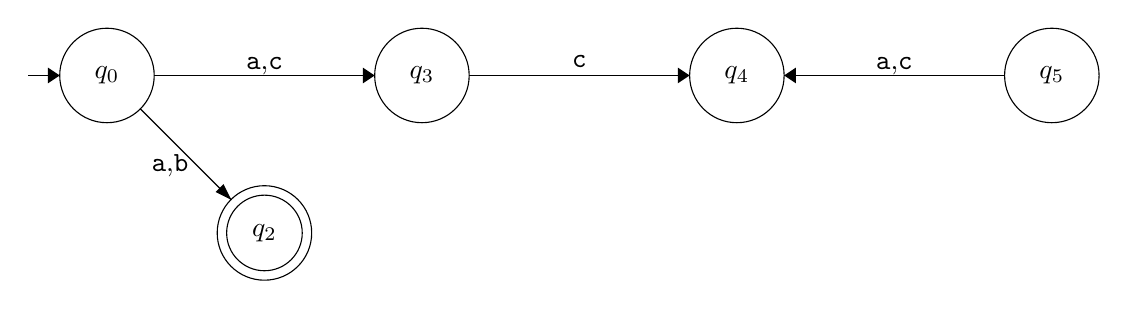
\begin{tikzpicture}[scale=0.2]
\tikzstyle{every node}+=[inner sep=0pt]
\draw [black] (-5,0) -- (-3,0);
\fill [black] (-3,0) -- (-3.75,-.5) -- (-3.75,.5);
\draw [black] (0,0) circle (3);
\draw (0,0) node {$q_0$};

\draw (10,0) node [above] {{\tt a},{\tt c}};
\draw [black] (3,0) -- (17,0);
\fill [black] (17,0) -- (16.25,-.5) -- (16.25,.5);
\draw [black] (20,0) circle (3);
\draw (20,0) node {$q_3$};

\draw (30,.5) node [above] {{\tt c}};
\draw [black] (23,0) -- (37,0);
\fill [black] (37,0) -- (36.25,-.5) -- (36.25,.5);
\draw [black] (40,0) circle (3);
\draw (40,0) node {$q_4$};

\draw (50,0) node [above] {{\tt a},{\tt c}};
\draw [black] (43,0) -- (57,0);
\fill [black] (43,0) -- (43.75,-.5) -- (43.75,.5);
\draw [black] (60,0) circle (3);
\draw (60,0) node {$q_5$};

\draw (4, -5) node [below] {{\tt a},{\tt b}};
\draw [black] (2.1,-2.1) -- (7.9,-7.9);
\fill [black] (7.9,-7.9) -- (6.9,-7.4) -- (7.4,-6.9);
\draw [black] (10,-10) circle (3);
\draw [black] (10,-10) circle (2.4);
\draw (10,-10) node {$q_2$};
\end{tikzpicture}

\end{figure}

Навіть при поверхневому аналізі діаграми переходів наведеного скінченого автомата видно, що вершини $q_3$, $q_4$ та $q_5$ є ``зайвими'', тобто при їх вилученні новий автомат буде еквівалентний початковому. З наведеного вище прикладу видно, що для отриманого детермінованого скінченого автомата можна запропонувати еквівалентний йому автомат з меншою кількістю станів, тобто мінімізувати скінчений автомат. Очевидно що серед зайвих станів цього автомата є недосяжні та тупикові стани.

\subsubsection{Недосяжні стани}

Стан $q$ скінченого автомата $M$ називається \textit{недосяжним}, якщо на діаграмі переходів скінченого автомата не існує шляху з $q_0$ в $q$. \medskip

\textbf{Алгоритм [пошуку недосяжних станів].} Спочатку спробуємо побудувати множину досяжних станів. Якщо $Q_m$ --- множина досяжних станів скінченого автомата $M$, то $Q \setminus Q_m$ --- множина недосяжних станів. Побудуємо послідовність множин $Q_0, Q_1, Q_2, \ldots$ таким чином, що:
\begin{enumerate}
	\item $Q_0 = \{q_0\}$.
	\item $Q_i = Q_{i-1} \cup \left\{ q \mid \exists a \in \Sigma, q_j \in Q_{i - 1}: q \in \delta(q_j, a) \right\}$.
	\item $Q_m = Q_{m+1} = \ldots$.
\end{enumerate}

Справді, очевидно, що кількість кроків скінчена, тому що послідовність $Q_i$ монотонна $\left(Q_0 \subseteq Q_1 \subseteq Q_2 \subseteq \ldots\right)$ та обмежена зверху: $Q_m \subseteq Q$. \medskip

Тоді $Q_m$ --- множина досяжних станів скінченого автомата, а $Q\setminus Q_m$ --- множина недосяжних станів. \medskip

Вилучимо з діаграми переходів скінченого автомата $M$ недосяжні вершини:
\begin{figure}[H]
	\centering
	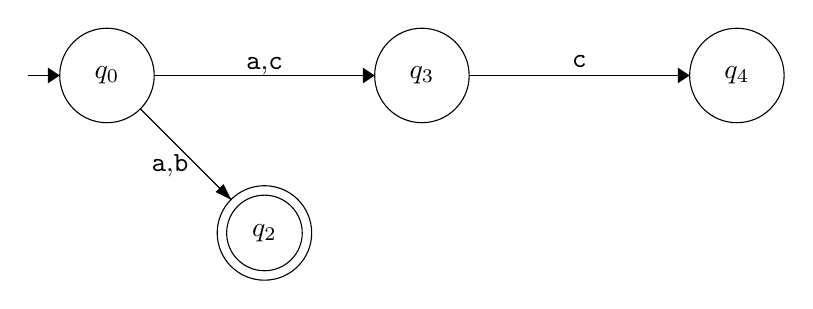
\begin{tikzpicture}[scale=0.2]
\tikzstyle{every node}+=[inner sep=0pt]
\draw [black] (-5,0) -- (-3,0);
\fill [black] (-3,0) -- (-3.75,-.5) -- (-3.75,.5);
\draw [black] (0,0) circle (3);
\draw (0,0) node {$q_0$};

\draw (10,0) node [above] {{\tt a},{\tt c}};
\draw [black] (3,0) -- (17,0);
\fill [black] (17,0) -- (16.25,-.5) -- (16.25,.5);
\draw [black] (20,0) circle (3);
\draw (20,0) node {$q_3$};

\draw (30,.5) node [above] {{\tt c}};
\draw [black] (23,0) -- (37,0);
\fill [black] (37,0) -- (36.25,-.5) -- (36.25,.5);
\draw [black] (40,0) circle (3);
\draw (40,0) node {$q_4$};

\draw (4, -5) node [below] {{\tt a},{\tt b}};
\draw [black] (2.1,-2.1) -- (7.9,-7.9);
\fill [black] (7.9,-7.9) -- (6.9,-7.4) -- (7.4,-6.9);
\draw [black] (10,-10) circle (3);
\draw [black] (10,-10) circle (2.4);
\draw (10,-10) node {$q_2$};
\end{tikzpicture}

\end{figure}

В новому автоматі функція $\delta$ визначається лише для досяжних станів. Побудований нами скінчений автомат з меншою кількістю станів буде еквівалентний початковому.

\subsubsection{Тупикові стани}

Стан $q$ скінченого автомата $M$ називається \textit{тупиковим}, якщо на діаграмі переходів скінченого автомата не існує шляху з $q$ в $F$. \medskip

\textbf{Алгоритм [пошуку тупикових станів].} Спочатку спробуємо знайти нетупикові стани. Якщо $S_m$ --- множина нетупикових станів, то $Q \setminus S_m$ --- множина тупикових станів. Побудуємо послідовність множин $S_0, S_1, S_2, \ldots$ таким чином, що:
\begin{enumerate}
	\item $S_0 = F$.
	\item $S_i = S_{i - 1} \cup \left\{ q \mid \exists a \in \Sigma: \delta(q, a) \cap S_{i - 1} \ne \varnothing \right\}$.
	\item $S_m = S_{m + 1} = \ldots$.
\end{enumerate}

Очевидно, що кількість кроків скінчена, тому що послідовність $S_i$ монотонна $\left(S_0 \subseteq S_1 \subseteq S_2 \subseteq \ldots\right)$ та обмежена зверху --- $S_m \subseteq Q$. \medskip

Тоді $S_m$ --- множина нетупикових станів скінченого автомата, а $Q \setminus S_m$ --- множина тупикових станів.  \medskip

Вилучимо з діаграми переходів скінченого автомата $M$ тупикові вершини:
\begin{figure}[H]
	\centering
	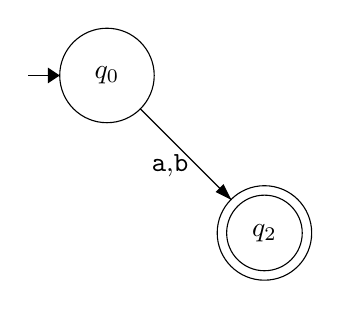
\begin{tikzpicture}[scale=0.2]
\tikzstyle{every node}+=[inner sep=0pt]
\draw [black] (-5,0) -- (-3,0);
\fill [black] (-3,0) -- (-3.75,-.5) -- (-3.75,.5);
\draw [black] (0,0) circle (3);
\draw (0,0) node {$q_0$};

\draw (4, -5) node [below] {{\tt a},{\tt b}};
\draw [black] (2.1,-2.1) -- (7.9,-7.9);
\fill [black] (7.9,-7.9) -- (6.9,-7.4) -- (7.4,-6.9);
\draw [black] (10,-10) circle (3);
\draw [black] (10,-10) circle (2.4);
\draw (10,-10) node {$q_2$};
\end{tikzpicture}

\end{figure}

В новому автоматі функція $\delta$ визначається лише для нетупикових станів.

\subsubsection{Еквівалентні стани}

Автомат, у котрого відсутні недосяжні та тупикові стани, піддається подальшій мінімізації шляхом ``склеювання'' еквівалентних станів. Продемонструємо це на конкретному прикладі:
\begin{figure}[H]
	\centering
	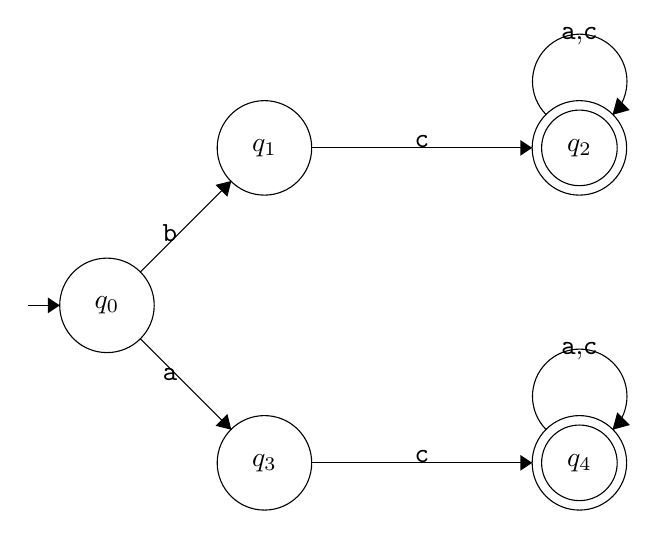
\begin{tikzpicture}[scale=0.2]
\draw [black] (-5,0) -- (-3,0);
\fill [black] (-3,0) -- (-3.75,-.5) -- (-3.75,.5);
\draw [black] (0,0) circle (3);
\draw (0,0) node {$q_0$};

\draw [black] (2.1, 2.1) -- (7.9,7.9);
\fill [black] (6.9,7.65) -- (7.9,7.9) -- (7.65,6.9);
\draw (4,4) node [above] {{\tt b}};
\draw [black] (10,10) circle (3);
\draw (10,10) node {$q_1$};

\draw [black] (2.1, -2.1) -- (7.9,-7.9);
\fill [black] (6.9,-7.65) -- (7.9,-7.9) -- (7.65,-6.9);
\draw (4,-4) node [below] {{\tt a}};
\draw [black] (10,-10) circle (3);
\draw (10,-10) node {$q_3$};

\draw [black] (13,10) -- (27,10);
\fill [black] (27,10) -- (26.25,10.5) -- (26.25,9.5);
\draw (20,10) node [above] {{\tt c}};
\draw [black] (30,10) circle (3);
\draw [black] (30,10) circle (2.4);
\draw (30,10) node {$q_2$};
\draw (27.9,12.1) arc (225:-45:3);
\fill [black] (32.1,12.1) -- (32.4,13.2) -- (33.2,12.4);
\draw (30,16.5) node [above] {{\tt a},{\tt c}};

\draw [black] (13,-10) -- (27,-10);
\fill [black] (27,-10) -- (26.25,-10.5) -- (26.25,-9.5);
\draw (20,-10) node [above] {{\tt c}};
\draw [black] (30,-10) circle (3);
\draw [black] (30,-10) circle (2.4);
\draw (30,-10) node {$q_4$};
\draw (27.9,-7.9) arc (225:-45:3);
\fill [black] (32.1,-7.9) -- (32.4,-6.8) -- (33.2,-7.6);
\draw (30,-3.5) node [above] {{\tt a},{\tt c}};
\end{tikzpicture}

\end{figure}

Очевидно, що для наведеного вище скінченого автомата можна побудувати еквівалентний йому скінчений автомат з меншою кількістю станів:
\begin{figure}[H]
	\centering
	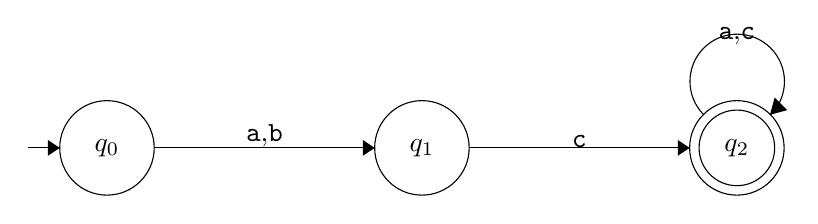
\begin{tikzpicture}[scale=0.2]
\draw [black] (-5,0) -- (-3,0);
\fill [black] (-3,0) -- (-3.75,-.5) -- (-3.75,.5);
\draw [black] (0,0) circle (3);
\draw (0,0) node {$q_0$};

\draw [black] (3,0) -- (17,0);
\fill [black] (16.25,.5) -- (17,0) -- (16.25,-.5);
\draw (10,0) node [above] {{\tt a},{\tt b}};
\draw [black] (20,0) circle (3);
\draw (20,0) node {$q_1$};

\draw [black] (23,0) -- (37,0);
\fill [black] (37,0) -- (36.25,.5) -- (36.25,-.5);
\draw (30,0) node [above] {{\tt c}};
\draw [black] (40,0) circle (3);
\draw [black] (40,0) circle (2.4);
\draw (40,0) node {$q_2$};
\draw (37.9,2.1) arc (225:-45:3);
\fill [black] (42.1,2.1) -- (42.4,3.2) -- (43.2,2.4);
\draw (40,6.5) node [above] {{\tt a},{\tt c}};
\end{tikzpicture}

\end{figure}

Ми досягли бажаного нам результату шляхом ``склеювання'' двох станів $q_1 \equiv q_3$ та $q_2 \equiv q_4$. \medskip

Два стани $q_1$ та $q_2$ скінченого автомата $M$ називаються \textit{еквівалентними} (позначається $q_1 \equiv q_2$), якщо множини слів, які розпізнає автомат, починаючи з $q_1$ та $q_2$, співпадають. \medskip

Нехай $q_1$ та $q_2$ --- два різні стани скінченого автомата $M$, а $x \in \Sigma^\star$. Будемо говорити, що ланцюжок $x$ \textit{розрізняє} стани $q_1$ та $q_2$, якщо $(q_1,x) \models^\star (q_3, \varepsilon)$ та $(q_2,x) \models^\star (q_4, \varepsilon)$, причому рівно один зі станів $q_3$ і $q_4$ (не) належить множині заключних станів. \medskip

Стани $q_1$ та $q_2$ називаються \textit{$k$-нерозрізнені}, якщо не існує ланцюжка $x$ $(\left|x\right| \le k)$, що розрізняє стани $q_1$ та $q_2$. \medskip

Два стани $q_1$ та $q_2$ \textit{нерозрізнені}, якщо вони $k$-нерозрізнені для довільного $k$. \medskip

\textbf{Теорема.} \textit{Два стани $q_1$ та $q_2$ довільного скінченого автомата $M$ з $n$ станами нерозрізнені, якщо вони $(n - 2)$-нерозрізнені.} \medskip

\textbf{Доведення:} На першому кроці розіб'ємо множину станів скінченого автомата на дві підмножини: $F$ та $Q \setminus F$. На цій основі побудуємо відношення $\equiv^0$: $q_1 \equiv^0 q_2$, якщо обидва стани одночасно належать $F$ або $Q \setminus F$. \medskip

Побудуємо відношення $\equiv^k$: $q_1 \equiv^k q_2$, якщо $q_1 \equiv^{k - 1} q_2$ та $\delta(q_1,a) \equiv^{k - 1} \delta(q_2, a)$ для всіх $a \in \Sigma$. \medskip

Очевидно, кожна побудована множина містить не більше $(n-1)$ елементи. \medskip

Таким чином, можна отримати не більше $(n-2)$ уточнення відношення $\equiv^0$. \medskip

Відношення $\equiv^{n - 2}$ визначає класи еквівалентних станів автомата $M$.

\subsubsection{Алгоритм}

\textbf{Алгоритм [побудови мінімального скінченого автомата].}
\begin{enumerate}
	\item Побудувати скінчений автомат без тупикових станів.
	\item Побудувати скінчений автомат без недосяжних станів.
	\item Знайти множини еквівалентних станів та побудувати найменший (мінімальний) автомат.
\end{enumerate}

\subsection{Контрольні запитання}

\begin{enumerate}
	\item Які автомати називаються еквівалентними? % ті які задають одну мову
	\item Який стан автомату називається недосяжним? % той у який немає шляху з $q_0$ на діаграмі переходів
	\item Опишіть алгоритм пошуку недосяжних станів і доведіть його збіжність. Бонус: оцініть складність цього алгоритму за часом і пам'яттю.
	\item Який стан автомату називається тупиковим? % той з якого немає шляху в $F$ на діаграмі переходів
	\item Опишіть алгоритм пошуку тупикових станів і доведіть його збіжність. Бонус: оцініть складність цього алгоритму за часом і пам'яттю.
	\item Які стани називаються еквівалентними? % для яких не існує розрізняючого слова
	\item Опишіть алгоритм пошуку еквівалентних станів і доведіть його збіжність. Бонус: оцініть складність цього алгоритму за часом і пам'яттю.
	\item Опишіть алгоритм мінімізації детермінованого скінченного автомату. Бонус: виведіть з попередніх оцінок складність цього алгоритму за часом і пам'яттю.
\end{enumerate}
